\documentclass[11pt]{article}

\usepackage{amsmath}
\usepackage{amssymb}
\usepackage{graphicx}
\usepackage{caption}
\usepackage{subcaption}

\topmargin -.5in
\textheight 9in
\oddsidemargin -.25in
\evensidemargin -.25in
\textwidth 7in

\newcommand{\code}[1]{\texttt{#1}}

\begin{document}

\author{Gu, Qiao}
\title{16-720B Homework 4 Write-up}
\maketitle

\medskip

\subsection*{Q1.1}

\newcommand{\intrinsic}{\mathbf{K}}
\newcommand{\fundamental}{\mathbf{F}}
\newcommand{\essential}{\mathbf{E}}
\newcommand{\homox}{\tilde{\mathbf{x}}}

Consider the point $\mathbf{w}$ where the principle axes of the two cameras intersect, and we can see that $\homox_1=[0,0,1]^T$ and $\homox_2=[0,0,1]^T$ corresponding one point in 3D. Therefore

\begin{align}
    \homox_2^T \essential \homox_1 =
    \begin{bmatrix}
        0 & 0 & 1
    \end{bmatrix}
    \begin{bmatrix}
        \essential_{11} & \essential_{12} & \essential_{13} \\
        \essential_{21} & \essential_{22} & \essential_{23} \\
        \essential_{31} & \essential_{32} & \essential_{33}
    \end{bmatrix}
    \begin{bmatrix}
        0 \\ 0 \\ 1
    \end{bmatrix}
    = \essential_{33} = 0
\end{align}

Since two cameras are normalized, the intrinsic matrices for them are identity:  $\intrinsic_1=\intrinsic_2=\mathbf{I}$.
Then $\essential = \intrinsic_1^T \fundamental \intrinsic_2 = \essential$.
Therefore, $\essential_{33} = \fundamental_{33}=0$.

% Suppose the intrinsic matrix for two cameras are
%
% \begin{align}
%     \intrinsic_1 =
%     \begin{bmatrix}
%         f_{1x} & \gamma_1 & 0 \\
%         0 & f_{1y} & 0 \\
%         0 & 0 & 1
%     \end{bmatrix}
%     \quad
%     \intrinsic_2 =
%     \begin{bmatrix}
%         f_{2x} & \gamma_2 & 0 \\
%         0 & f_{2y} & 0 \\
%         0 & 0 & 1
%     \end{bmatrix}
% \end{align}

% \begin{align}
%     \essential = \intrinsic_1^T \fundamental \intrinsic_2 &=
%     \begin{bmatrix}
%         f_{1x} & 0 & 0 \\
%         \gamma_1 & f_{1y} & 0 \\
%         0 & 0 & 1
%     \end{bmatrix}
%     \begin{bmatrix}
%         \fundamental_{11} & \fundamental_{12} & \fundamental_{13} \\
%         \fundamental_{21} & \fundamental_{22} & \fundamental_{23} \\
%         \fundamental_{31} & \fundamental_{32} & \fundamental_{33}
%     \end{bmatrix}
%     \begin{bmatrix}
%         f_{2x} & \gamma_2 & 0 \\
%         0 & f_{2y} & 0 \\
%         0 & 0 & 1
%     \end{bmatrix}
%     \\
%     &= \begin{bmatrix}
%         f_{1x} & 0 & 0 \\
%         \gamma_1 & f_{1y} & 0 \\
%         0 & 0 & 1
%     \end{bmatrix}
%     \begin{bmatrix}
%         \dots & \dots & \fundamental_{13} \\
%         \dots & \dots & \fundamental_{23} \\
%         \dots & \dots & \fundamental_{33} \\
%     \end{bmatrix}
%     =
%     \begin{bmatrix}
%         \dots & \dots & \dots \\
%         \dots & \dots & \dots \\
%         \dots & \dots & \fundamental_{33} \\
%     \end{bmatrix}
% \end{align}

\newpage

\subsection*{Q1.2}

\newcommand {\rotation} {\mathbf{R}}
\newcommand {\translation} {\mathbf{t}}
\newcommand {\bl} {\mathbf{l}}

Suppose the cameras are normalized in the sense that their intrinsic matrices are both identity:  $\intrinsic_1=\intrinsic_2=\mathbf{I}$.

Now that the translation and rotation from camera 1 to camera 2 are

\begin{align}
    \rotation =
    \begin{bmatrix}
        1 & 0 & 0 \\
        0 & 1 & 0 \\
        0 & 0 & 1
    \end{bmatrix}, \quad
    \translation =
    \begin{bmatrix}
        t_x \\ 0 \\ 0
    \end{bmatrix}
\end{align}

And thus the essential matrix are

\begin{align}
  \essential=\translation_\times \rotation=
  \begin{bmatrix}
    0 & 0 & 0 \\
    0 & 0 & -t_x \\
    0 & t_x & 0
  \end{bmatrix}
\end{align}

Therefore for an epipolar line in camera 1 $\bl_1^T \homox_1=0$ and $\homox_2^T \essential \homox_1 =0$, where $\homox_2$ is a fixed point on the image plane of camera 2 resulting from the ray corresponding to the epipolar line, then we can see that

\begin{align}
  \bl_1^T = \homox_2^T \essential =
  \begin{bmatrix}
    x_2 & y_2 & 1
  \end{bmatrix}
  \begin{bmatrix}
    0 & 0 & 0 \\
    0 & 0 & -t_x \\
    0 & t_x & 0
  \end{bmatrix}
  =
  \begin{bmatrix}
    0 & t_x & -t_x y_2
  \end{bmatrix}
\end{align}

Similarly we can see that any epipolar line in camera 1 has $\bl_2^T = [0 \; -t_x \; t_xy_1]$. Since the first elements in both $\bl_1$ and $\bl_2$ are zero, the epipolar lines are parallel to $x$ axis.

% According to the dfinition of essential matrix
%
% \begin{align}
%     \homox_2^T \translation \times \rotation \homox_1 &=
%     \homox_2^T \translation_\times \rotation \homox_1 =
%     \homox_2^T
%     \begin{bmatrix}
%         0 & 0 & 0 \\
%         0 & 0 & -t_x \\
%         0 & t_x & 0 \\
%     \end{bmatrix}
%     \begin{bmatrix}
%         1 & 0 & 0 \\
%         0 & 1 & 0 \\
%         0 & 0 & 1
%     \end{bmatrix}
%     \homox_1
%     \\ &=
%     \homox_2^T
%     \begin{bmatrix}
%         0 & 0 & 0 \\
%         0 & 0 & -t_x \\
%         0 & t_x & 0 \\
%     \end{bmatrix}
%     \homox_1 =
%     \begin{bmatrix}
%         x_2 & y_2 & 1
%     \end{bmatrix}
%     \begin{bmatrix}
%         0 \\ -t_x \\ t_x y_1
%     \end{bmatrix}
%     \\ &=
%     -t_x y_2 + t_x y_1 = 0
%     \\ & \Rightarrow
%     y_1 = y_2
% \end{align}
%
% For a certain epipolar line in camera 2, it has a fixed epipole with fixed $y_1$ in camera 1, and thus every 3D point on the corresponding incident ray to camera 1 has a projection with a fixed $y_2=y_1$ in camera 2, which means the epipolar line has a fixed $y$ coordinate, and thus parallel to x-axis.
%
% The above deduction also holds if camera 1 and 2 are exchanged.

\newpage

\subsection*{Q1.3}

\newcommand{\pointw}{\mathbf{w}}

Assume $(\rotation_i, \translation_i)$ and $(\rotation_i, \translation_i)$ are the rotation and translation from the world coordinate frame to the camera coordinate frame at time $i$ and time $j$. And suppose $\rotation_{rel}$ and $\translation_{rel}$ are the rotation and translation from camera at time $i$ to the camera at time $j$. Then for a point $\pointw$ in the 3D world

\begin{align}
    & \lambda_i \homox_i = \rotation_i \pointw + \translation_i, \quad
    \lambda_j \homox_j = \rotation_j \pointw + \translation_j
    \nonumber \\ \Rightarrow &
    \pointw = \rotation_i ^T (\lambda_i \homox_i - \translation_i)
    \nonumber \\ \Rightarrow &
    \lambda_j \homox_j = \rotation_j \rotation_i ^T (\lambda_i \homox_i - \translation_i) + \translation_j
    \nonumber \\ \Rightarrow &
    \lambda_j \homox_j = \rotation_j \rotation_i ^T \lambda_i \homox_i - \rotation_j \rotation_i ^T \translation_i + \translation_j
    \nonumber \\ \Rightarrow &
    \lambda_j \homox_j = \lambda_i \rotation_{rel} \homox_i + \translation_{rel}
\end{align}

Therefore

\begin{align}
    \rotation_{rel} = \rotation_j \rotation_i ^T, \quad
    \translation_{rel} = \translation_j - \rotation_j \rotation_i ^T \translation_i
\end{align}

Then the essential and fundamental matrix can be derived as

\begin{align}
  \essential &= (\translation_{rel})_\times \rotation_{rel} \\
  \fundamental &= (\intrinsic^{-1})^T \fundamental \intrinsic^{-1} = (\intrinsic^{-1})^T (\translation_{rel})_\times \rotation_{rel} \intrinsic^{-1}
\end{align}

\newpage

\subsection*{Q1.4}

\newcommand {\bv} {\mathbf{v}}
\newcommand {\bH} {\mathbf{H}}
\newcommand {\bI} {\mathbf{I}}
\newcommand {\bw} {\mathbf{w}}

Suppose the mirror is orthogonal to a unit vector $\bv$ pointing in to the mirror, then we can have the Householder transformation matrix $\bH=\bI - 2\bv\bv^T$. Suppose the real world coordinate has its origin at a point on the mirror, then for any point $\bw$ in the world coordinate, the mirror produce its reflection $\bw_2=\bH\bw_1=\bw_1 - 2\bv\bv^T\bw_1=\bw_1 + 2\alpha\bv$, where $\alpha=-\bv^T\bw_1$ is the dixed distance from $\bw_2$ to the mirror.

This two points in 3D produce two point on the image plane as follows

\begin{align}
  \lambda_1\homox_1 &= \bw_1 \\
  \lambda_2\homox_2 &= \bw_2 = \bw_1 + 2\alpha\bv
\end{align}

This is equivalent to a two-camera system where $\rotation=\bI$ and $\translation=2\alpha\bv$. Therefore

\begin{align}
  \essential = \translation_\times \rotation = 2\alpha\bv_\times \bI=2\alpha\bv_\times
\end{align}

is skew-symmetric. Since there are only one camera with only one intrinsic $\intrinsic$, for fundamental matrix

\begin{align}
  \fundamental = (\intrinsic^{-1})^T \essential \essential^{-1}
  \fundamental^T = (\intrinsic^{-1})^T \essential^T \essential^{-1} = -(\intrinsic^{-1})^T \essential \essential^{-1} = -\fundamental
\end{align}

Therefore the fundamental matrix $\fundamental$ of this equivalent two-camera system is symmetric.

\newpage

\subsection*{Q2.1}

The fundamental matrix $\fundamental$ given by the 8-point algorithm is

\begin{verbatim}
[[ 9.80213861e-10 -1.32271663e-07  1.12586847e-03]
 [-5.72416248e-08  2.97011941e-09 -1.17899320e-05]
 [-1.08270296e-03  3.05098538e-05 -4.46974798e-03]].
\end{verbatim}

And visualization result is shown in Figure.~\ref{fig:q2.1}

\begin{figure}[h!]
    \centering
    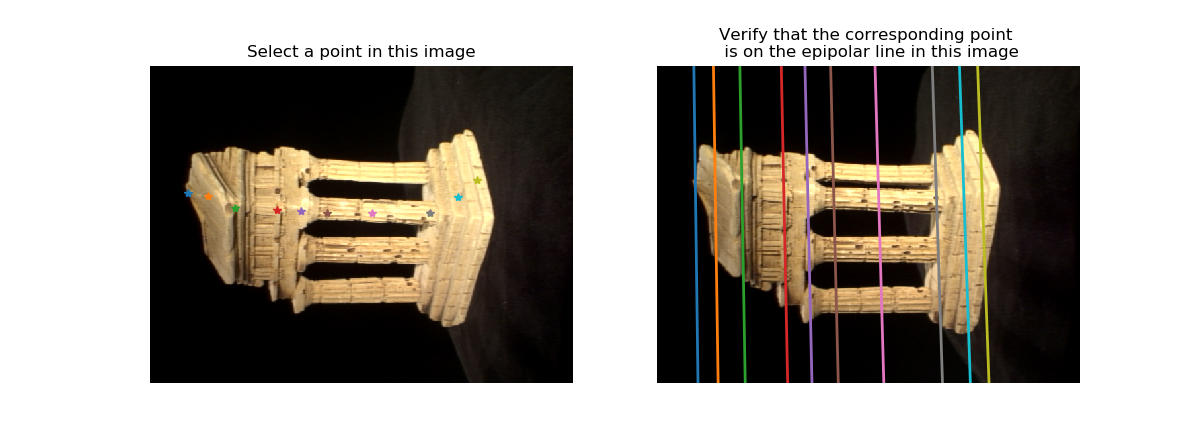
\includegraphics[width=.8\linewidth]{../results/q2_1.png}
    \caption{The visualization results showing the fundamental matrix given by 8-point algorithm. }
    \label{fig:q2.1}
\end{figure}

\newpage

\subsection*{Q2.2}





\end{document}
